\documentstyle[12pt,psfig,draft,lscape,array,longtable]{nature-ejb}
%\documentstyle[12pt,psfig,lscape,array,longtable]{nature-ejb}

\textwidth16.15cm\textheight24.cm\voffset-1.cm\hoffset+1.5cm

\def\simlt{\mathrel{\hbox{\rlap{\hbox{\lower4pt\hbox{$\sim$}}}\hbox{$<$}}}}
\def\simgt{\mathrel{\hbox{\rlap{\hbox{\lower4pt\hbox{$\sim$}}}\hbox{$>$}}}}

\def\ale{\mathrel{\hbox{\rlap{\hbox{\lower4pt\hbox{$\sim$}}}\hbox{$<$}}}}
\def\age{\mathrel{\hbox{\rlap{\hbox{\lower4pt\hbox{$\sim$}}}\hbox{$>$}}}}

\def\nodata{---}

\def\ra#1#2#3{#1$^{\rm h}$#2$^{\rm m}$#3$^{\rm s}$}
\def\dec#1#2#3{$#1^\circ#2'#3''$}

\newcommand{\hst}{\textit{HST}}
\newcommand{\swift}{\textit{Swift}}
\newcommand{\ergcms}{erg cm$^{-2}$ s$^{-1}$}
\newcommand{\uJy}{\mbox{$\mu$Jy}}
\newcommand{\Tburst}{\mbox{$T_{\rm GRB}$}}

\def\spose#1{\hbox to 0pt{#1\hss}}

\begin{document}

\begin{center}
{\Large SUPPLEMENTARY INFORMATION} \\
%{\large The Birth of a Relativistic Outflow in the Unusual
%$\gamma$-ray Transient Swift\,J164449.3+573451} \\
%{\large A.~Zauderer et al.}
\end{center}

\headertitle{Supplementary Information}
\mainauthor{Zauderer et al.}


\section{Archival Radio Non-detections of Swift\,J164449.3+573451}

We inspected the location of Swift\,J164449.3+573451 in archival 1.4
GHz images from the NRAO VLA Sky Survey (NVSS) taken in March 1995,
and the Faint Images of the Radio Sky at Twenty-cm (FIRST) survey
taken in July 1998.  No counterpart is detected to $3\sigma$ limits of
about $1.5$ mJy and 0.45 mJy, respectively.  The non-detections place
an upper bound on the radio luminosity of 
$6\times~10^{30}$~erg~s$^{-1}$~Hz$^{-1}$ (March 1995) and 
$2\times~10^{30}$~erg~s$^{-1}$~Hz$^{-1}$ (July 1998), 
thereby ruling out radio-loud AGN activity
(typically\cite{mpm90} $\simgt~10^{33}$~erg~s$^{-1}$~Hz$^{-1}$).


\section{Expanded Very Large Array Observations}
\label{sec:evla}

We observed Swift\,J164449.3+573451 with the EVLA beginning 0.82~d
after the $\gamma$-ray trigger (see Table~\ref{tab:radio}). We used
the EVLA's new Wideband Interferometric Digital Architecture (WIDAR)
correlator to obtain up to 2~GHz of bandwidth at several frequencies.
At all frequencies, we used 3C286 for bandpass and flux calibration.
Absolute flux calibration is accurate to $\sim$~10$\%$.
At 1.4~GHz, we used J1634+6245 for phase calibration.  For phase
calibration at all other frequencies, we used J1638+5720 and also
included a third calibrator, J1639+5357, at 5.8~GHz.
Polarization calibration was not performed.  The data were
reduced and imaged with the Astronomical Image Processing System
(AIPS) software package.


\section{AMI Large Array observations}
\label{sec:ryle}

We observed with 6 antennas of the AMI Large
Array (Mullard Radio Astronomy Observatory, Cambridge, UK) at 15.4 GHz
with a bandwidth of 3.75~GHz beginning 2.79~d after the $\gamma$-ray
trigger (see Table~\ref{tab:radio}).  The maximum baseline is about
110~m and the angular resolution is 25~arcsec.  Observations ranged in
duration from 45~min to 11~hr.  Observations of the compact source
J1638+5720 were interleaved at intervals of 10 m as a phase reference,
and the flux density scale was established by regular observations of
the calibrators 3C48 and 3C286.  Absolute flux calibration is
accurate to better than 10$\%$.  The AMI array uses linearly-polarized 
feeds and measures Stokes I+Q.  It does not measure any other combination 
of Stokes parameters.  Polarization calibration is not reported here.  

\section{Owens Valley Radio Observatory 40-m Observations}
\label{sec:ovro40}

We observed Swift\,J164449.3+573451 with the OVRO 40-meter telescope
at a frequency of 15~GHz beginning 2.82~d after the $\gamma$-ray
trigger (see Table~\ref{tab:radio}).  The 40-m telescope is equipped
with a dual-beam Dicke-switched receiver with two symmetric, off-axis
beams (each 2.5~arcmin full-width at half-maximum) separated
azimuthally by 12.95~arcmin.  The receiver has a 2.5~GHz
noise-equivalent reception bandwidth.  We used sky switching,
alternating the source between the two beams to reduce atmospheric and
ground pickup, and to account for the non-identical nature of the two
beams.  See Ref.~\pcite{ovro} for further details of the telescope
and receiver system.  The flux scale is derived from observations of 
3C286 using standard spectral models and coefficients\cite{baars}
 with an absolute uncertainty of $\sim$~$5\%$.

We note that daytime measurements of Swift\,J164449.3+573451 lead to
consistently discrepant flux densities, most likely due to increased
thermal emission from the ground.  These discrepant measurements, as
quoted in an initial GCN circular, have been used
elsewhere$^{5}$ to argue for a short variability timescale in
the radio emission, and hence a large Lorentz factor of 
$\Gamma\simgt$~10.  We do not support this conclusion, 
and indeed, as we show in
Section~\ref{sec:synch}, $\Gamma\simgt$~10 appears to lead to a
non-self consistent model.


\section{Combined Array for Research in Millimeter Astronomy
Observations}
\label{sec:carma}

We observed Swift\,J164449.3+573451 with CARMA beginning 1.85 d after
the $\gamma$-ray trigger (see Table~\ref{tab:radio}).  CARMA is a
heterogeneous array comprised of nine 6.1-m antennas and six 10.4-m
antennas.  Observations were taken at a rest frequency of 87.3 and
93.6 GHz with a total bandwidth ranging between 6.8 and 7.8~GHz.  We
used Neptune as our primary flux calibrator, and J1824+568 and
J1638+573 as bandpass and phase calibrators, respectively.  The
overall uncertainty in the absolute flux calibration is $\sim 15\%$.
Data calibration and imaging were done with the MIRIAD software
package.


\section{Submillimeter Array Observations}
\label{sec:sma}

We observed Swift\,J164449.3+573451 with the Submillimeter Array (SMA;
Ref.~\pcite{hml04}) beginning 0.28 d after the burst, followed by
monitoring at $\sim 1.3$ mm and $\sim 0.9$ mm (see
Table~\ref{tab:radio}).  Observations were made using at least seven
of the eight antennas, in a wide range of weather conditions, with
$\tau_{\rm 225}$ ranging from 0.04 to 0.3.  For each observation, the
full 8~GHz (4~GHz in each sideband separated by 10~GHz) were combined
to increase the signal-to-noise ratio.  The data were calibrated using
the MIR software package developed at Caltech and modified for the
SMA, while for imaging and analysis we used MIRIAD.  Gain calibration
was performed using J1642+689, 3C345, and J1849+670.  Absolute flux
calibration was performed using real-time measurements of the system
temperatures, with observations of Neptune to set the scale, accurate
to within $\sim$ 10 $\%$.
Bandpass calibration was done using 3C454.3, J1924-292, and 3C279.


\section{Very Long Baseline Array Observations}
\label{sec:vlba}

We observed Swift\,J164449.3+573451 with the NRAO Very Long Baseline
Array (VLBA) and the 100 m Effelsberg telescopes starting on 2011
April 2.25~UT for a duration of 7~hr at 8.4 and 22~GHz.  The
observations were performed with eight frequency bands of 8~MHz
bandwidth each in dual circular polarization, resulting in a total
data rate of 512 Mbps. We used J1638+5720, located only 0.92$^\circ$
from Swift\,J164449.3+573451, as a phase-referencing source at both
frequencies.  At 22 GHz, sources were switched every 40 seconds, while
at 8.4 GHz we spent 40 seconds on the calibrator and 90 seconds on
target.  A second calibrator, J1657+5705, was also observed for six
minutes at each frequency to check the calibration of the data.  We
also employed\cite{brf05,rmb+09} $\sim 30$~min of geodetic blocks at
the start and end of the observations for atmospheric calibration.  

The data were data were correlated at the VLBA Array Operations Center
in Socorro, New Mexico, and calibrated\cite{kvr+06} using AIPS and
ParselTongue.  We applied the latest values of the Earth's orientation
parameters, and performed zenith delay corrections based on the
results of the geodetic block observations.  Total electron content
maps of the ionosphere were used to correct for ionospheric phase
changes.  Amplitude calibration used system temperature measurements
and standard gain curves.  We performed ``manual phase-calibration''
using the data from one scan of J1638+5720 to remove instrumental
phase offsets among the frequency bands.  We then fringe fitted the
data from J1638+5720.  Since J1638+5720 shows extended structure, we
performed phase self-calibration first, and then amplitude and phase
self-calibration to construct robust models at both frequencies.  The
calibration was transferred to the target source and J1657+5705.
Residual phase calibration errors were removed by performing one round
of phase self-calibration on the target with a solution interval of 30
min. The data were imaged in AIPS using robust weighting (ROBUST=0).

The 8.4 GHz images were restored with a beam of $1.03\times 0.46$~mas
at a position angle of $-29^\circ$.  We achieved a noise level of 30
$\mu$Jy beam$^{-1}$, which is close to the expected thermal noise
limit.  Swift\,J164449.3+573451 was detected with a flux density of
$1.71\pm 0.03$ mJy beam$^{-1}$.  The 22 GHz images were restored with
a beam of $0.44\times 0.24$ mas at a position angle of $2^\circ$.  We
achieved a noise level of 120 $\mu$Jy beam$^{-1}$, which is twice the
expected thermal noise limit.  Swift\,J164449.3+573451 was detected
with a flux density of $4.68\pm 0.12$ mJy~beam$^{-1}$.
Absolute flux calibration is $\sim$~15-20$\%$.

The position of the source at both frequencies was measured from the
purely phased referenced image (without phase self-calibration on the
target).  The formal uncertainties of the positions are 
$\approx 3-8$~$\mu$as.  The true uncertainty is dominated by systematic errors
induced from residual atmospheric effects and an opacity effect
(``core shift'') in the calibrator source. The position difference
between the two frequencies is 61~$\mu$as in right ascension and 
33~$\mu$as in declination.  The absolute position as determined from the
22~GHz image is $\alpha_{\rm J2000}=$\ra{16}{44}{49.93130},
$\delta_{\rm J2000}=$\dec{+57}{34}{59.6893} with an uncertainty of 
0.1~mas ($68\%$ confidence level) in each coordinate.

The limit of 0.25~mas corresponds to $r\simlt 2\times 10^{18}$~cm.
This places an upper bound on the Lorentz factor of $\Gamma\simlt 15$
(for relativistic expansion with $r\approx\Gamma^2ct$ and a start time
of 2011 March 25).  Alternatively, we can use the inferred Lorentz
factor of $\Gamma\sim 2$ to place an upper bound on the lifetime of
the source of $\simlt 1.5$ yr.


\section{Optical Spectroscopy}
\label{sec:opt}

We obtained two spectra of the host galaxy of Swift\,J164449.3+573451.
The first spectrum was a 7200 s observation taken at a mean time of
2011 April 1.34 UT using Hectospec on the 6.5-m MMT and covered the
observed wavelength range $3700-9150$ \AA.  The second one was taken
in nod-and-shuffle mode using GMOS on the 8-m Gemini-North telescope
on 2011 April 4.62 UT (program GN-2011A-Q-4).  The R400 grating was
used to cover the wavelength range $4930-9180$ \AA.

The spectra are consistent with each other and exhibit the usual
narrow emission lines of a star-forming galaxy ${\rm [OII]}\lambda
3727$, H$\beta$, ${\rm [OIII]}\lambda\lambda 4959,5007$, H$\alpha$) at
a redshift of $z=0.354$.  Neither spectrum shows any evidence for a
broad (${\rm FWHM}\simgt 1000$~km~s$^{-1}$) component to the H$\alpha$
line (SI Figure~\ref{fig:host}b), as would be seen in a
Seyfert 1 galaxy (i.e., a galaxy with an unobscured actively-accreting
central massive black hole).  To examine the possibility that the host
of Swift\,J164449.3+573451 contained a central black hole that was
actively accreting prior to the current outburst, but which was
obscured from our line of sight, we examined the ratios of several
emission lines.  Galaxies whose emission lines are powered by the
ionizing radiation field of young stars can be separated from those
powered by the harder radiation field produced by accretion onto a
massive black hole using an excitation diagram\cite{bpt81} (SI
Figure~\ref{fig:host}a).  The host galaxy of Swift\,J164449.3+573451
is clearly located in the portion of the diagram associated with
star-forming galaxies and not AGN.  A small systematic uncertainty
results from our inability to adequately correct for the underlying
stellar absorption features with the signal-to-noise ratio of our
current spectra, but that effect will only move the point associated
with Swift\,J164449.3+573451 down and to the left, closer to the main
locus of star-forming galaxies.  In addition, neither of our spectra
show any evidence for emission from high-excitation lines such as
${\rm [NeV]}\lambda\lambda 3345,3425$, which would be evidence for an
AGN.  In summary, the spectra of the host galaxy of
Swift\,J164449.3+573451 are consistent with expectations for a galaxy
whose central black hole was not actively accreting prior to the
current outburst.


\section{Synchrotron Model of the Radio Emission}
\label{sec:synch}

We assume that the radiation observed from Swift\,J164449.3+573451 in
the radio band corresponds to synchrotron emission from relativistic
electrons in a spherically expanding source.  We use as inputs the
observations at $\Delta t\approx 5$, 10, 15, and 22~d (see Figure~2 of
the main text).  Given the shape of the spectrum we use $\nu_a\approx
\nu_p$ in all three epochs.

We use the methods described in \S3 of Ref.~\pcite{kn09} to analyze
each epochs independently.  Although that work deals with gamma-ray
bursts, which are highly relativistic, the basic framework is quite
general.  We describe the source by means of five parameters: the
source radius, $r$, the bulk Lorentz factor, $\Gamma$, the Lorentz
factor of the relativistic electrons that produce the radiation at the
synchrotron peak, $\gamma_e$ (in the source frame), the number of
relativistic electrons, $N_e$, and the magnetic field strength $B$ (in
the source frame).  To determine these five parameters, we need five
constraints.  Three of these are provided by the measured values of
$\nu_p$, $F_{\nu,p}$, and $\nu_a$, coupled with equations 1, 2, and
15 in Ref.~\pcite{kn09}.

A fourth condition is obtained by the assumption that the magnetic
field and the relativistic particles are in equipartition.  We write
this condition as (see equations 33 and 34 Ref.~\pcite{kn09}):
\begin{equation}
E_B = B^2 r^3/2 = 10\,E_e = 10\,N_e\gamma_e\Gamma m_ec^2, 
\label{RN1}
\end{equation}
where the factor of 10 assumes that the total thermal energy in both
electrons and protons is 10 times that in electrons alone. 

Finally, for the fifth condition, we require the radius of the source
to be consistent with ballistic expansion from the moment of the
initial burst.  The observed time of $\Delta t=5$~d corresponds to a
time of 3.7~d in the frame.  Due to relativistic time compression, the
actual time that the source would have expanded is $(3.7\,{\rm
d})/(1-\beta)$, where $\beta=v/c$ is the relativistic bulk expansion
velocity of the source.  Thus, the assumption of ballistic motion
requires:
\begin{equation}
r = (3.7\,{\rm d})\times \beta c/(1-\beta). 
\label{RN2}
\end{equation}

Using the above five conditions, we obtain solution for the relevant
parameters of the source at all four epochs.  These solutions are
summarized in Table~\ref{tab:model}.  We find that all four epochs
lead to the same expansion velocity of $\Gamma\approx 1.2$ (i.e., no
deceleration) and an energy of $E_B = 10\,E_e\approx 1.6\times
10^{50}$ erg.  The outflow mass, $8\times 10^{-5}$ M$_\odot$, combined
with the constant expansion velocity, indicate that the density of the
swept-up medium is $\simlt 3\times 10^3$~cm$^{-3}$.

Fitting a linear trend to the expanding source size (as indicated by
the data), we can estimate the initial formation date of the
relativistic outflow (Figure~\ref{fig:vel}).  We find that the this
date is 2011 March $23-26$ UT, in excellent agreement with
the initial {\it Swift} detection of $\gamma$-ray emission on 2011
March 25 UT.  This indicates that the formation of the relativistic
outflow indeed coincided with the initial accretion episode onto the
supermassive black hole.

Using the model, we have computed the synchrotron self-Compton (SSC)
emission and find that the peak occurs at $\approx 0.1$ keV and the
luminosity at the peak is $\approx 2\times 10^{45}$~erg~s$^{-1}$.
These values do not agree with the observed X-ray spectrum which peaks
beyond 1 keV and has a peak luminosity of $\approx 10^{47}$~erg~s$^{-1}$ 
(observer frame).  Thus, the model developed here suggests
that the X-rays must arise either from a process other than SSC (e.g.,
Compton scattering of external radiation) or from a different region
of the source.

Interestingly, in the framework of this model relativistic expansion
with $\Gamma\sim 10$, as seen in most blazars, is ruled out.  For
$\Gamma\sim 10$, the radius $r$ required to fit the observed radio
flux and spectrum is much smaller than the radius implied by ballistic
dynamics.  It may be possible to avoid this difficulty by modeling the
source as a highly collimated jet.  However, the collimation angle of
the jet would need to be much smaller than $1/\Gamma$, which is
unlikely to be true.  Another approach is to give up the condition of
energy equipartition.


\clearpage
\begin{center}
%\begin{longtable}[t]
%\begin{tabular}{l>{\setlength\hsize{0.67\hsize}}cccc}
\begin{longtable}{lcccc}
\caption{Summary of Radio Observations} 
\label{tab:radio} \\
%\multicolumn{5}{c}{Summary of Radio Observations}\\
\hline
\hline
UT Date & $\Delta t$ & Facility & $\nu$ & $F_\nu$ \\
        & (d)        &          & (GHz) & (mJy)   \\\hline
\endfirsthead
\hline
\hline
UT Date & $\Delta t$ & Facility & $\nu$ & $F_\nu$ \\
        & (d)        &          & (GHz) & (mJy)   \\\hline
\endfirsthead
\endhead
%
Mar 31.28   &  2.74  & EVLA & 1.4 & $<0.30$  \\
Apr 1.28    &  3.74  & EVLA & 1.4 & $<0.18$  \\\hline
%
Mar 31.28   &  2.74  & EVLA & 1.8 & $<0.15$  \\
Apr 1.28    &  3.74  & EVLA & 1.8 & $<0.15$  \\\hline
%
Mar 29.36   &  0.82  & EVLA & 4.9 & $0.25\pm 0.01$  \\
Mar 30.25   &  1.71  & EVLA & 4.9 & $0.34\pm 0.02$  \\
Mar 30.49   &  1.95  & EVLA & 4.9 & $0.34\pm 0.02$  \\
Mar 31.28   &  2.74  & EVLA & 4.9 & $0.61\pm 0.02$  \\
Apr 1.27    &  3.73  & EVLA & 4.9 & $0.82\pm 0.02$  \\
Apr 2.26    &  4.72  & EVLA & 4.9 & $1.48\pm 0.02$  \\
Apr 4.28    &  6.74  & EVLA & 4.9 & $1.47\pm 0.02$  \\
Apr 9.47    &  11.93 & EVLA & 4.9 & $1.80\pm 0.03$  \\
Apr 17.27   &  19.73 & EVLA & 4.9 & $2.11\pm 0.01$  \\\hline
%
Mar 29.36   &  0.82  & EVLA & 6.7 & $0.38\pm 0.01$  \\
Mar 30.25   &  1.71  & EVLA & 6.7 & $0.63\pm 0.02$  \\
Mar 30.49   &  1.95  & EVLA & 6.7 & $0.64\pm 0.02$  \\
Mar 31.28   &  2.74  & EVLA & 6.7 & $1.16\pm 0.02$  \\
Apr 1.27    &  3.73  & EVLA & 6.7 & $1.47\pm 0.02$  \\
Apr 2.26    &  4.72  & EVLA & 6.7 & $1.50\pm 0.02$  \\
Apr 4.28    &  6.74  & EVLA & 6.7 & $2.15\pm 0.02$  \\
Apr 9.47    &  11.93 & EVLA & 6.7 & $3.79\pm 0.03$  \\
Apr 17.27   &  19.73 & EVLA & 6.7 & $3.44\pm 0.01$  \\\hline
%
Apr 9.46    &  11.92  & EVLA & 8.4 & $5.49\pm 0.09$  \\\hline
%
Mar 31.33   &  2.79  & AMI-LA & 15.0 & $2.80\pm 0.45$ \\
Apr 1.18    &  3.65  & AMI-LA & 15.0 & $3.58\pm 0.23$ \\
Apr 2.16    &  4.62  & AMI-LA & 15.0 & $4.35\pm 0.28$ \\
Apr 3.10    &  5.56  & AMI-LA & 15.0 & $5.10\pm 0.36$ \\
Apr 4.10    &  6.56  & AMI-LA & 15.0 & $6.67\pm 0.51$ \\
Apr 5.33    &  7.79  & AMI-LA & 15.0 & $6.65\pm 0.48$ \\
Apr 6.10    &  8.56  & AMI-LA & 15.0 & $7.36\pm 0.45$ \\
Apr 8.03    &  10.49 & AMI-LA & 15.0 & $8.30\pm 0.24$ \\
Apr 8.39    &  10.85 & AMI-LA & 15.0 & $7.01\pm 0.13$ \\
Apr 9.12    &  11.58 & AMI-LA & 15.0 & $8.50\pm 0.32$ \\
Apr 13.20   &  15.66 & AMI-LA & 15.0 & $8.66\pm 0.40$ \\
Apr 14.27   &  16.73 & AMI-LA & 15.0 & $9.91\pm 0.63$ \\
Apr 16.33   &  18.79 & AMI-LA & 15.0 & $10.96\pm 0.89$ \\
Apr 17.30   &  19.76 & AMI-LA & 15.0 & $10.78\pm 0.77$ \\\hline
%
Mar 31.37   & 2.82  & OVRO40 & 15.0 & $2.36\pm 1.14$ \\
Apr 1.34    & 3.80  & OVRO40 & 15.0 & $3.17\pm 1.17$ \\
Apr 8.36    & 10.82 & OVRO40 & 15.0 & $8.06\pm 0.95$ \\
Apr 10.36   & 12.82 & OVRO40 & 15.0 & $7.65\pm 0.90$ \\
Apr 12.33   & 14.79 & OVRO40 & 15.0 & $7.45\pm 0.80$ \\
Apr 12.41   & 14.87 & OVRO40 & 15.0 & $6.60\pm 1.22$ \\
Apr 15.35   & 17.81 & OVRO40 & 15.0 & $10.54\pm 0.93$ \\
Apr 19.33   & 21.79 & OVRO40 & 15.0 & $11.99\pm 1.03$ \\
Apr 21.36   & 23.82 & OVRO40 & 15.0 & $9.55\pm 1.04$ \\\hline
%
Mar 30.24   & 1.70 & EVLA & 19.1 & $2.12\pm 0.02$   \\
Apr 1.24    & 3.70 & EVLA & 19.1 & $4.36\pm 0.05$   \\
Apr 2.26    & 4.72 & EVLA & 19.1 & $5.25\pm 0.03$   \\
Apr 3.36    & 5.82 & EVLA & 19.1 & $6.38\pm 0.05$   \\
Apr 4.27    & 6.73 & EVLA & 19.1 & $5.31\pm 0.03$   \\
Apr 16.38   & 18.84 & EVLA & 19.1 & $12.01\pm 0.03$  \\\hline
%				   	 	   
Mar 30.24   & 1.70 & EVLA & 24.4 & $3.01\pm 0.03$   \\
Apr 1.24    & 3.70 & EVLA & 24.4 & $5.58\pm 0.06$   \\
Apr 2.26    & 4.72 & EVLA & 24.4 & $6.70\pm 0.03$   \\
Apr 3.36    & 5.82 & EVLA & 24.4 & $7.88\pm 0.12$   \\
Apr 4.27    & 6.73 & EVLA & 24.4 & $6.60\pm 0.03$   \\
Apr 16.38   & 18.84 & EVLA & 24.4 & $12.69\pm 0.03$  \\\hline
%
Mar 31.28   & 2.70 & EVLA & 44 & $6.35\pm 0.10$  \\
Apr 1.24    & 3.70 & EVLA & 44 & $7.71\pm 0.08$  \\
Apr 3.36    & 5.82 & EVLA & 44 & $9.38\pm 0.08$  \\\hline
%
Apr 2.68    & 5.14  & CARMA & 87 & $18.6\pm 0.3$   \\
Apr 3.63    & 6.09  & CARMA & 87 & $21.7\pm 0.2$   \\
Apr 4.72    & 7.18  & CARMA & 87 & $14.6\pm 0.4$   \\
Apr 6.63    & 9.09  & CARMA & 87 & $15.1\pm 0.2$   \\
Apr 12.15   & 14.61 & CARMA & 87 & $10.4\pm 0.2$   \\
Apr 16.60   & 19.06 & CARMA & 87 & $9.36\pm 0.5$   \\
Apr 19.61   & 22.07 & CARMA & 87 & $5.49\pm 0.3$   \\\hline
%
Mar 30.39   & 1.85  & CARMA & 94 & $15.7\pm 0.3$   \\
Apr 16.60   & 19.06 & CARMA & 94 & $10.7\pm 1.0$   \\\hline
%
Apr 13.66   & 16.12 & SMA & 200 & $14.1\pm 1.5$    \\
Apr 18.70   & 21.16 & SMA & 200 & $8.2\pm 1.2$     \\
Apr 20.74   & 23.20 & SMA & 200 & $7.4\pm 1.0$     \\\hline
%
Mar 28.82   & 0.28  & SMA & 225 & $<33$            \\
Apr 4.74    & 7.20  & SMA & 225 & $14.9\pm 1.5$    \\
Apr 5.40    & 7.86  & SMA & 225 & $11.7\pm 0.4$    \\
Apr 11.63   & 14.10 & SMA & 225 & $13.3\pm 1.5$    \\
Apr 12.66   & 15.12 & SMA & 225 & $9.9 \pm 1.4$    \\
Apr 14.65   & 17.11 & SMA & 225 & $8.2 \pm 1.4$    \\
Apr 15.67   & 18.13 & SMA & 225 & $8.3 \pm 2.2$    \\\hline
%
Mar 30.39   & 1.85 & SMA & 345   & $35.1\pm 1.0$  \\
Mar 31.39   & 1.85 & SMA & 345   & $<10.2$        \\
Apr 1.71    & 4.17 & SMA & 345   & $<8.7$         \\\hline
%\enddata
%\end{deluxetable}
%\end{tabular}
\caption[]{Radio observations of Swift\,J164449.3+573451.  All values
of $\Delta t$ are relative to the $\gamma$-ray trigger.  For times
relative to the initial detection (2011 March 25 UT) as used in the
main text add 3.54 d.  Flux measurement errors are one standard
deviation systematic errors.  Absolute flux scaling depends on the
instrument.  See SI text for details.}
\label{tab:radio}
\end{longtable}
\end{center}


\clearpage
\begin{center}
\begin{longtable}{lcccc}
\caption{Summary of Radio SED Modeling} \\
\hline
\hline
Parameter & $\Delta t=5$ d & $\Delta t=10$ d & $\Delta t=15$ d  & $\Delta t=22$ d \\
\hline
\hline
$\nu_a=\nu_p$ (GHz; rest-frame)  & 600 & 250 & 140 & 80   \\
$F_{\nu,p}$ (mJy; rest-frame)    & 80  & 40  & 30  & 25   \\\hline 
$r$ ($10^{16}$ cm)               & 1.0 & 1.7 & 2.6 & 4.7  \\
$\Gamma$                         & 1.2 & 1.2 & 1.1 & 1.2     \\
$\beta$                          & 0.5 & 0.5 & 0.5 & 0.5      \\
$\gamma_e$                       & 150 & 140 & 140 & 140      \\
$B$ (G)                          & 17  & 8   & 4.6 & 2.6      \\
$N_e$ ($10^{53}$)                & 1.0 & 1.1 & 1.5 & 2.6      \\
$n_e$ (10$^4$ cm$^{-3}$)       & 2.4 & 0.5 & 0.2 & 0.06     \\
$E_B=10E_e$ ($10^{50}$ erg)      & 1.4 & 1.5 & 1.9 & 2.9      \\
$\theta_s$ ($\mu$as)             & 0.6 & 1.0 & 1.5 & 2.6      \\\hline 
\caption[]{Summary of relativistic model results for the four
broad-band SEDs shown in Figure 2 of the main text.  The top portion
lists the observed synchrotron parameters, while the bottom portion
lists the model fit results.}
\label{tab:model}
\end{longtable}
\end{center}


\clearpage
\begin{figure}[h!]
\centerline{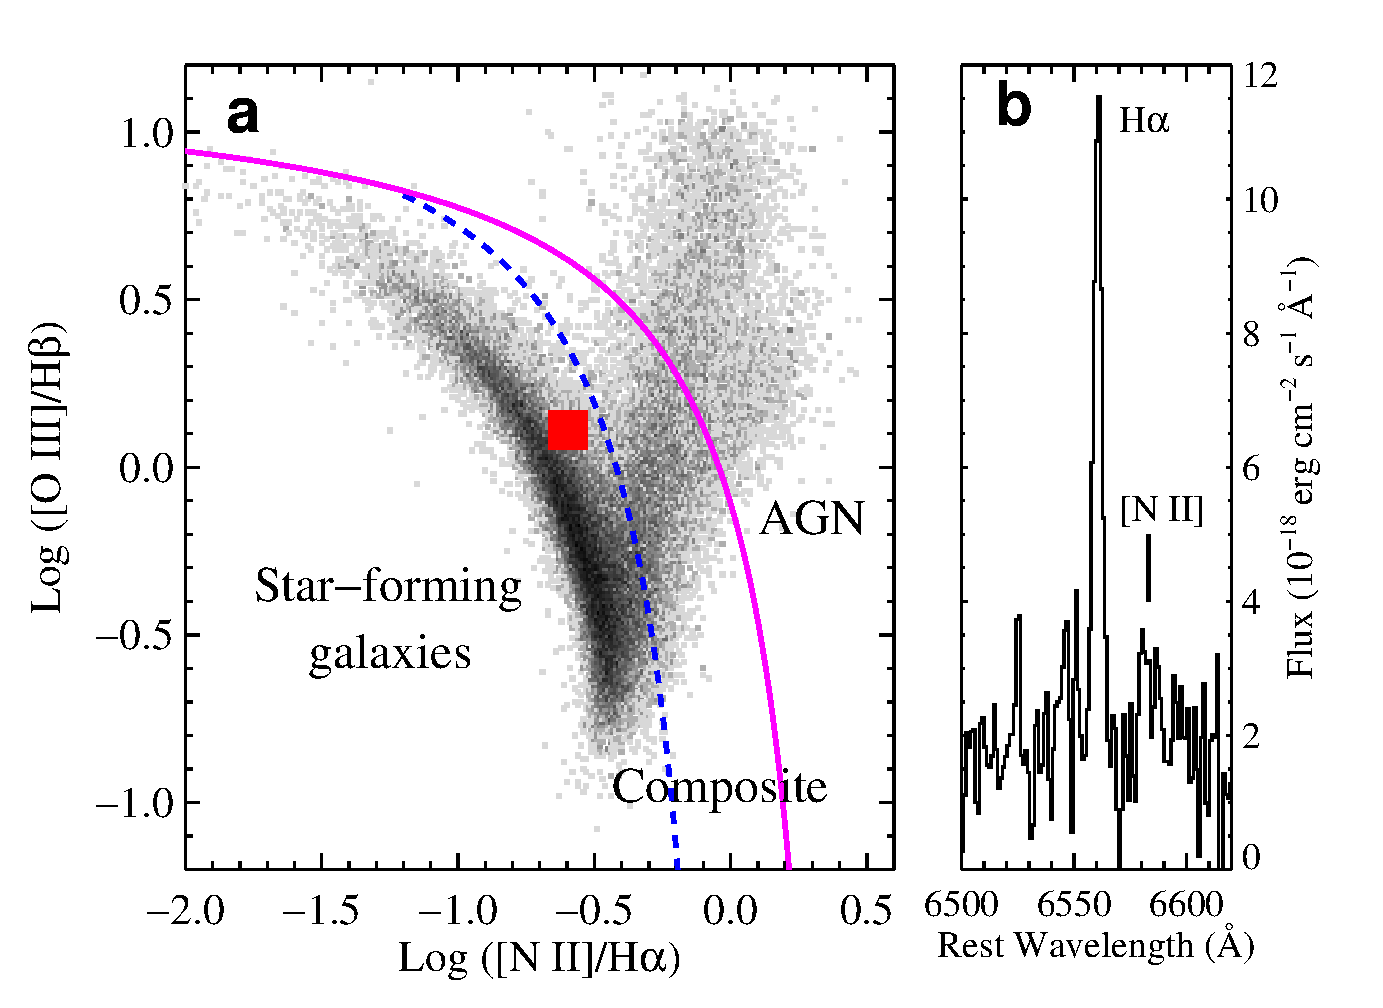
\psfig{file=si_hostprop.eps,width=6.5in,angle=0}}
\caption[]{\small Optical spectroscopy of the host galaxy of 
Swift\,J164449.3+573451 shows no indication of AGN activity.
(a) Excitation diagram comparing the
observed line ratios of the host galaxy of Swift\,J164449.3+573451 to
a sub-sample of galaxies observed\cite{kht+03,thk+04} in the Sloan
Digital Sky Survey.  The emission lines in objects found to the right
of the magenta line are powered by accretion onto massive black holes,
while those between the blue dashed line and the solid magenta line
show\cite{kgk+06} ``composite'' spectra of star formation plus AGN
activity.  Objects to the left of both lines have emission lines
dominated\cite{kgk+06} by star formation activity.  The host galaxy
(red square) is clearly in the portion of the diagram associated with
star-forming galaxies.  (b) The region around the H$\alpha$
line in the Gemini spectrum.  No broad component is observed as would
be expected for an active Seyfert 1 galaxy.}
\label{fig:host} 
\end{figure}


\clearpage
\begin{figure}
\centerline{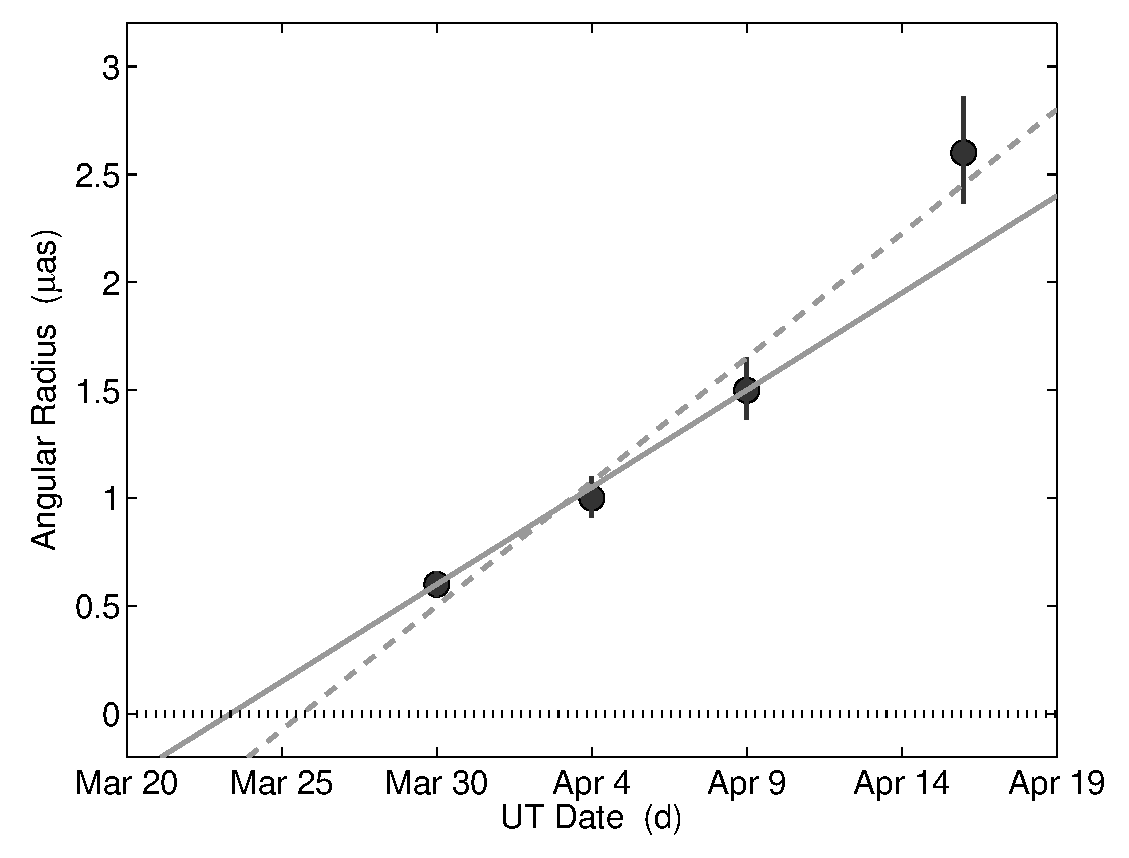
\psfig{file=figure2_si.eps,width=6.5in,angle=0}}
\caption[]{\small The radius of the radio emitting region inferred
from the relativistic model indicates a formation date in excellent 
agreement with the intial burst.  Angular radius of the
radio emitting region as a function of UT date.  The linear
growth in source size indicates a formation date of 2011 March 23-26
UT, in agreement with the initial {\it Swift}
detection of $\gamma$-ray emission on 2011 March 25 UT.  The solid and
dashed lines indicate fits to the first three epochs and all four
epochs, respectively.  We note that the last epoch on 2011 April 16 UT
has a larger uncertainty than the preceding measurements.}
\label{fig:vel} 
\end{figure}



\clearpage
\begin{thebibliography}{10}

\bibitem[{Miller}, {Peacock} \& {Mead}<22>]{mpm90} {Miller}, L.,
{Peacock}, J.~A.  \& {Mead}, A.~R.~G. {The bimodal radio luminosity
function of quasars}.  \newblock {\it Mon.~Not.~R.~Astr.~Soc.} {\bf
244}, 207--213 (1990).

% This reference is number 5 in the main text.
%\bibitem[{Bloom} {\it et~al.}<5>]{bgm+11} {Bloom}, J.~S., {Giannios},
%D., {Metzger}, B.~D., {Cenko}, S.~B., {Perley}, D.~A. {\it et al.} {A
%relativistic jetted outburst from a massive black hole fed by a
%tidally disrupted star}.  \newblock {\it ArXiv:1104.3257}, (2011).

\bibitem[{Richards} {\it et~al.}<23>]{ovro} {Richards}, J.~L., 
{Max-Moerbeck}, W., {Pavlidou}, V., {King}, O.~G. {\it et al.}
{Blazars in the {\it Fermi} Era:  The OVRO 40-m Telescope
Monitoring Program}. \newblock {\it ArXiv:1011.3111} (2011).

\bibitem[{Baars} {\it et~al.}<24>]{baars} {Baars}, J.~W.~M., {Genzel}, R.,
{Pauliny-Toth}, I.~I.~K., \& {Witzel}, A. {The Absolute Spectrum of Cas A - 
An Accurate Flux Density Scale and a Set of Secondary Calibrators}.
\newblock {\it Astron.~Astrophys.} {\bf 61}, 99--106 (1977).

\bibitem[{Ho}, {Moran} \& {Lo}<25>]{hml04} {Ho}, P.~T.~P., {Moran},
J.~M.  \& {Lo}, K.~Y. {The Submillimeter Array}.  \newblock {\it
Astrophys.~J.}  {\bf 616}, L1--L6 (2004).

\bibitem[{Brunthaler}, {Reid} \& {Falcke}<26>]{brf05} {Brunthaler}, A.,
{Reid}, M.~J.  \& {Falcke}, H. in {\it Future Directions in High
Resolution Astronomy} (ed {J.~Romney \& M.~Reid}) 455 (2005).

\bibitem[{Reid} {\it et~al.}<27>]{rmb+09} {Reid}, M.~J., {Menten},
K.~M., {Brunthaler}, A., {Zheng}, X.~W., {Moscadelli}, L. {\it et al.}
{Trigonometric Parallaxes of Massive Star-Forming Regions. I.  S 252
\& G232.6+1.0}.  \newblock {\it Astrophys.~J.} {\bf 693}, 397--405
(2009).

\bibitem[{Kettenis} {\it et~al.}<28>]{kvr+06} {Kettenis}, M., {van
Langevelde}, H.~J., {Reynolds}, C.  \& {Cotton}, B. in {\it
Astronomical Data Analysis Software and Systems XV} (ed {C.~Gabriel,
C.~Arviset, D.~Ponz, \& S.~Enrique}) 497 (2006).

\bibitem[{Baldwin}, {Phillips} \& {Terlevich}<29>]{bpt81} {Baldwin},
J.~A., {Phillips}, M.~M.  \& {Terlevich}, R. {Classification
parameters for the emission-line spectra of extragalactic objects}.
\newblock {\it Publ.~Astr.~Soc.~Pacific} {\bf 93}, 5--19 (1981).

\bibitem[{Kumar} \& {Narayan}<30>]{kn09} {Kumar}, P. \& {Narayan},
R. {GRB 080319B: evidence for relativistic turbulence, not internal
shocks}.  \newblock {\it Mon.~Not.~R.~Astr.~Soc.} {\bf 395}, 472--489
(2009).

\bibitem[{Kauffmann} {\it et~al.}<31>]{kht+03} {Kauffmann}, G.,
{Heckman}, T.~M., {Tremonti}, C., {Brinchmann}, J., {Charlot}, S. {\it
et al.} {The host galaxies of active galactic nuclei}.  \newblock {\it
Mon.~Not.~R.~Astr.~Soc.} {\bf 346}, 1055--1077 (2003).

\bibitem[{Tremonti} {\it et~al.}<32>]{thk+04} {Tremonti}, C.~A.,
{Heckman}, T.~M., {Kauffmann}, G., {Brinchmann}, J., {Charlot},
S. {\it et al.} {The Origin of the Mass-Metallicity Relation: Insights
from 53,000 Star-forming Galaxies in the Sloan Digital Sky Survey}.
\newblock {\it Astrophys.~J.} {\bf 613}, 898--913 (2004).

\bibitem[{Kewley} {\it et~al.}<33>]{kgk+06} {Kewley}, L.~J., {Groves},
B., {Kauffmann}, G.  \& {Heckman}, T. {The host galaxies and
classification of active galactic nuclei}.  \newblock {\it
Mon.~Not.~R.~Astr.~Soc.} {\bf 372}, 961--976 (2006).

\end{thebibliography}


\end{document}

